% Si vous vous demandez à quoi servent les empty \mbox après les paragraphes,
% vous êtes des boulays, apprenez latex.
\subsection{Définitions}
  \paragraph{Graphe} Un graphe est constitué d'un ensemble de points, et d'un ensemble
  d'arêtes (ou d'arcs, dans le cas orienté) qui relient ces points.

  \paragraph{Graphe connexe} Un graphe est dit connexe quand on peut aller de
  n'importe quel point vers n'importe quel autre point en suivant des arrêtes.

  \paragraph{Graphe complet} Un graphe est dit complet quand tout
  ses sommets sont reliés deux à deux par une arrête. Le nombre de d'arêtes
  d'un tel graphe est alors $\frac {n(n-1)} 2$.

  \paragraph{Degré d'un sommet} Le degré d'un sommet est le nombre d'arêtes
  incidentes à ce sommet.

\subsection{Modélisation mathématique}
Il existe plusieurs moyens de représenter des graphes. Parmi ceux-ci,
le plus simple est la matrice d'adjacence, où l'on stocke une matrice
de taille $n\times n$ ($n$ étant le nombre de sommets), dont chaque
colonne et chaque rangée représente un sommet. La case $i, j$ de la
matrice contient un $1$ si les sommets $i$ et $j$ sont reliés par une
arête (ou un arc dans le bon sens, dans le cas orienté). Évidemment,
cette représentation est loin d'être efficace, la mémoire utilisée
étant exponentielle quand le nombre de sommets du graphe
augmente. Toutefois, elle peut servir pour certains
algorithmes. Notamment, un algorithme de recherche de chemin peut
multiplier la matrice d'adjacence par elle-même $m$ fois : alors, il
existera un chemin de taille $m$ entre deux sommets si la case
correspondante contient un $1$.

  On peut également représenter les graphes par une liste de sommets,
  chacun ayant une liste d'arêtes.
  En mémoire, cette structure est donc constituée d'une liste de pointeurs
  vers des sommets. Les sommets contenant une liste de pointeurs vers des
  arêtes. Chaque arête dispose d'un pointeur vers chaque sommet extrémité.
  Cette structure est évidemment plus efficace, car elle ne stocke que
  les informations nécessaires.


\subsection{Graphes eulériens}
  \subsubsection{Analyse mathématique}
    Un graphe eulérien est un graphe contenant un cycle eulérien, c'est-à-dire
    une chaîne parcourant toutes les arêtes du graphe une et une seule fois, en
    revenant au sommet de départ.

    \paragraph{Théorème d'Euler} Un graphe connexe est eulérien si et seulement
    si chacun de ses sommets est de degré pair.

    \paragraph{}
    Un graphe semi-eulérien, quant à lui, contient une chaîne eulérienne:
    celle-ci passe également par toutes les arêtes du graphe une seule et
    unique fois, mais ne retourne pas au point de départ. Le théorème précédent
    se généralise alors aux graphes semi-eulériens: un graphe connexe est
    semi-eulérien si et seulement tous ses sommets sauf deux sont associés à un
    nombre pair d'arêtes. Dans ce cas, la chaîne eulérienne aura pour départ
    l'un des deux sommets associés à un nombre impair d'arêtes et pour point
    d'arrivée le deuxième.

  \subsubsection{Méthode de résolution}
    Afin de trouver une chaîne ou un cycle eulérien dans un graphe, on peut
    utiliser deux méthodes: une méthode qui teste toutes les possibilités, et
    une autre plus intelligente et moins coûteuse.

    \paragraph{Matrices latines}
      La première méthode est inspirée des matrices latines. Chaque coefficient
      de la matrice sera un ensemble de chaînes, une chaîne étant elle-même une
      liste de sommets. La matrice latine de notre graphe sera la matrice $M$
      dont chaque coefficient $m_{i,j}$ vaudra:
      \begin{itemize}
        \item l'ensemble vide si le nœud $i$ n'est pas relié au nœud $j$ dans
          le graphe;
        \item un ensemble contenant pour unique élément la chaîne  $[N_i,N_j]$
          si les nœuds $i$ et $j$ sont reliés (où $N_k$ représente le nœud
          $k$).
      \end{itemize}

      Nous définissions ensuite un produit sur les coefficients d'une telle
      matrice. Le produit de deux chaînes sera:
      \begin{itemize}
        \item nul si le dernier nœud de la première chaîne n'est pas le premier
          nœud du deuxième;
        \item la concaténation des deux chaînes sinon.
      \end{itemize}

      Le produit de deux ensembles de chaînes sera l'ensemble contenant les
      produits de chaque couple de nœuds.

      Pour tout $k$ entier naturel, le coefficient $(i,j)$ de la matrice $M^k$
      représentera l'ensemble des chaînes de longueur $k$ reliant les nœuds $i$
      et $j$.

      Puisque une chaîne eulérienne passe une unique fois par chaque arête, il
      suffira de calculer la matrice latine élevée à cette puissance pour
      trouver sur sa diagonale l'ensemble des cycles possibles. En éliminant à
      chaque produit les chaînes qui passent plusieurs fois par la même arête,
      on trouve l'ensemble des cycles eulériens.

      La complexité de cet algorithme est exponentielle, calculer la puissance
      de la matrice latine revient en fait à calculer chaque chaîne possible dans
      le graphe, et tester si elle est un cycle eulérien ou non.

    \paragraph{Algorithme d'Euler}
      La deuxième méthode, basée sur l'algorithme d'Euler est nettement plus
      efficace. Une fonction récursive cherche un cycle eulérien d'un
      sous-graphe de notre graphe de départ, puis s'appelle récursivement sur
      chacun des sommets parcourus par cette chaîne, dans le graphe où l'on a
      supprimé les arêtes déjà parcourues. En reconstruisant ces cycles
      astucieusement, on parvient à trouver un cycle eulérien de complexité
      linéaire en le nombre d'arêtes du graphe.

  \subsubsection{Algorithmes}
    \paragraph{Méthode de la matrice latine} \mbox{}
      \begin{lstlisting}
Entrée : un graphe
Sortie : la liste des cycles eulériens dans le cas d'un graphe eulérien
         la liste des chaînes eulériennes dans le cas d'un graphe semi-eulérien
         la liste vide sinon

Construire la matrice latine du graphe :
    construire une matrice à n lignes et n colonnes
    remplir la matrice de listes vides
    pour chaque nœud du graphe:
        pour chaque arête sortant de ce nœud:
            ajouter la liste [noeud de départ, noeud d'arrivée] à la case de la matrice correspondante

n = "le nombre d'arêtes total du graphe"

calculer la puissance (n-1)ième de la matrice

pour chaque coefficient de la matrice ainsi calculée:
    si le coefficient n'est pas nul:
        concaténer ce coefficient à la variable de retour
      \end{lstlisting}

    \paragraph{Produit matriciel} \mbox{}
      \begin{lstlisting}
Entrée : A et B deux matrices latines
Sortie : le produit de ces deux matrices

construire la matrice de retour à n lignes et n colonnes
initialiser chaque coefficient de cette matrice à la liste vide

pour chaque coefficient de la matrice de retour:
    pour k allant de 1 jusqu'à n:
        calculer les chaînes produits entre a(i,k) et b(k,j)
        ajouter au coefficient de la matrice ces chaînes
      \end{lstlisting}

    \paragraph{Produit entre listes de chaînes (coefficients de matrices
    latines)} \mbox{}
      \begin{lstlisting}
Entrée : liste_1 et liste_2 deux listes de chaîne
Sortie : une liste de chaînes

créer une liste de chaîne vide (liste de retour)
pour i dans liste_1:
    pour j dans liste_2:
        construire la chaîne résultante de la concaténation de i et j (en enlevant le nœud présent deux fois)
        construire un ensemble de chaîne vide
        pour k allant de 1 à la longueur de la chaîne construit:
            construire la chaîne élémentaire menant du nœud k au nœud k+1
            si cette chaîne n'est pas dans l'ensemble:
                ajouter cette chaîne dans l'ensemble
            sinon:
                rendre la chaîne nulle
                sortir de la boucle

        si le chaîne n'est pas nulle:
                concaténer la chaîne trouvée à la liste de retour
retourner la liste de retour
			\end{lstlisting}

\subsection{Graphes hamiltoniens}
  \subsubsection{Analyse mathématique}
    Un graphe (semi-)hamiltonien est un graphe sur lequel on peut
    trouver un cycle (ou une chaîne) passant par tout les sommets une et une
    seule fois. Ce problème est donc celui d'un enfant qui souhaiterait visiter
    de manière unique toutes les salles d'un musée.

    Le problème de savoir si un graphe est (semi-)hamiltonien est NP-complet,
    de même que de trouver un cycle ou une chaîne s'il y en a.

    Il existe cependant des conditions suffisantes pour lesquelles on peut
    affirmer qu'un graphe est hamiltonien.

    \paragraph{Théorème} Un graphe complet est hamiltonien. C'est une
    conséquence du théorème de Dirac.

    \paragraph{Théorème de Dirac} Un graphe simple à $n$ sommets ($n \ge 3$)
    dont chaque sommet est au moins de degré $\frac{n}{2}$ est hamiltonien.

    \paragraph{Théorème de Ore} Un graphe simple à $n$ sommets ($n \ge 3$) tel
    que la somme des degrés de toute paire de sommets non adjacents vaut au
    moins $n$ est hamiltonien.

    \paragraph{Théorème de Pósa} Un graphe simple à $n$ sommets ($n \ge 3$) est
    hamiltonien si:
    \begin{itemize}
      \item pour tout entier $k$ tel que $1 \le k < \frac{n-1}{2}$ le nombre de
        sommets de degré inférieur ou égal à $k$ est inférieur à $k$;
      \item le nombre de sommets de degré inférieur ou égal à $\frac{n-1}{2}$
        est inférieur ou égal à $\frac{n-1}{2}$.
    \end{itemize}

    \paragraph{Fermeture d'un graphe} La fermeture d'un graphe est
    le graphe construit à partir de celui en rajoutant des arrêtes entre chaque
    sommets $a$ et $b$ tel que $\deg(a)+\deg(b) > n$ tant qu'il en existe.

    \paragraph{Théorème de Bondy et Chvátal} Un graphe est hamiltonien si et
    seulement si sa fermeture est hamiltonienne.

    Ce théorème n'est utile que si l'on peut utiliser l'un des théorèmes
    précédents sur la fermeture.

  \subsubsection{Méthode de résolution}
    Pour tester si un graphe est hamiltonien on peut utiliser les théorèmes
    précédents. Si le graphe ne respecte les conditions d'aucun de ces
    théorèmes, on recherche une chaîne hamiltonienne dans ce graphe.

    Pour rechercher une chaîne hamiltonienne dans un graphe, on pourrait
    chercher parmi toutes les chaînes possibles. La complexité d'un tel
    algorithme dans le pire des cas est donc très mauvaise: $O(n!)$. Comme on
    peut s'arrêter dès qu'on a trouvé une chaîne sans devoir tester toutes les
    autres chaînes possibles, la complexité moyenne sera inférieure.

  \subsubsection{Algorithmes}
    \paragraph{Tests de semi-hamiltoniannité} \mbox{}
      \begin{lstlisting}
Entrée : un graphe
Sortie : un booléen indiquant si le graphe est semi-hamiltonien ou non

si le graphe suit les conditions du théorème de Dirac ou du théorème de Pósa:
    retourner Vrai
sinon:
    chercher une chaîne hamiltonienne
    retourner Vrai si on en a trouvé un, Faux sinon
      \end{lstlisting}

    \paragraph{Recherche de chaîne hamiltonienne} \mbox{}
      \begin{lstlisting}
Entrée : un graphe graph
         un point de départ optionnel node_from
         un ensemble (éventuellement vide) de nœuds déjà parcouru nodes_done
Sortie : une chaîne hamiltonienne sous la forme d'une liste ordonnée de points, ou None s'il n'en existe pas

Si la fonction a été appelée sans node_from:
    node_from = "un nœud de graph"

ajouter node_from à nodes_dones

si cardinal(node_from) == ordre(graph):
    retourner [node_from]

pour chaque arête dans le graphe:
    autre = "le point opposé à node_from par rapport à cette arête"
    si autre dans nodes_done:
        passer à la prochaîne arête

    appeler la fonction récursivement avec graphe, node_from et nodes_dones comme paramètre
    si la liste retournée est non-vide:
        y ajouter node_from au début et la retourner

retourner None (si on arrive ici, aucunne chaîne n'est bonne)
      \end{lstlisting}

\subsection{Problème du voyageur de commerce}\label{sec:tsp}
  \subsubsection{Analyse mathématique}
    Le problème du voyageur de commerce consiste à chercher un chemin passant
    par tous les sommets du graphe, de longueur minimale.
    Ce problème peut s'illustrer par l'exemple d'une
    fraiseuse qui doit percer des trous dans une plaque le plus
    rapidement possible, ou encore par un car de touristes qui souhaiterait
    trouver l'itinéraire le plus rapide pour visiter un certain nombre de lieux.

    On peut modéliser ce problème par un graphe complet, dont les arêtes ont un
    coût qui correspond à la distance entre chaque point, on cherche alors le
    cycle hamiltonien de coût minimal. On sait qu'un tel cycle existe car le
    graphe est complet.

    Cependant trouver un tel cycle est un problème NP-complet~: il n'existe
    donc pas d'algorithme efficace pour trouver ce cycle, à part une recherche
    exhaustive.
    En effet, la seule méthode exacte consisterait à tester toutes les chaînes
    hamiltoniennes, et à prendre celle la plus courte, mais le nombre de chaînes
    hamiltonniennes croît exponentiellement en fonction du nombre de sommets
    dans le graphe.

    Nous allons donc nous concentrer sur les méthodes approchées de résolution,
    qui peuvent donner de très bons résultats tout en étant rapides.
    Toutefois, le résultat n'est donc pas forcément le plus court.

  \subsubsection{Heuristiques}
    Les heuristiques vont nous permettre de construire un chemin court (par
    rapport au plus court possible), de manière rapide, avec le moins de calcul
    possible.  Étant donné qu'on est confronté à énormément de possibilités
    pendant la recherche, elles vont permettre d'orienter cette dernière, en
    faisant des choix les plus judicieux possibles sur les possibilités à
    explorer.

    \paragraph{Exemple} Une heuristique simple consiste à partir d'un sommet au
    hasard du graphe et d'aller au sommet le plus proche sur lequel on n'est
    pas encore passé (puis à retourner au sommet de départ pour boucler le
    cycle). Cet algorithme est en $O(n)$ et donc rapide. Mais il n'offre
    cependant aucune garantie de résultat, il existe même des graphes pour
    lesquels il donne le pire cycle.

    Plus généralement, chercher parmi les $p$ sommets les plus proches s'avère
    être une solution relativement efficace, avec une complexité en $O(p^n)$
    (donc toujours exponentielle si $p \neq 1$).

    Une méthode purement basée sur cette heuristique consisterait donc à parcourir
    tout le graphe, en allant sur le voisin le plus proche du sommet courant~:

    \begin{lstlisting}
Entrée : g (Graphe complet)
Sortie : (coût, cycle) où cycle est un cycle hamiltonien construit selon la méthode du plus proche voisin et coût son coût associé sous forme de liste de points
coût = 0
cycle = ["un point de g au hasard"]

tant qu'il reste des points:
    # On ajoute au cycle le point suivant
    plus_proche = "point de g sur lequel on est pas encore passé le plus proche du dernier point du cycle"

    coût += "coût de plus_proche au dernier point du cycle"
    cycle = cycle :: plus_proche

# On ferme le cycle
coût += "coût du dernier au premier point de cycle"
cycle = cycle :: "premier point de chaîne"

retourner (coût, cycle)
    \end{lstlisting}

  \subsubsection{Recherche locale}

    Les heuristiques nous donnant des solutions acceptables, choisies avec un
    minimum de «~bon sens~», il est ensuite possible de tenter d'améliorer
    ces solutions, via de la recherche locale.
    Partant d'une solution fournie, on va explorer les solutions voisines
    à cette dernière, afin de voire si on pourrait pas trouver des solutions
    encore meilleures parmi leur voisinage.

    \paragraph{Exemple} Un algorithme de recherche locale adapté au problème
    du voyageur de commerce est le 2-opt.
    Le principe du 2-opt consiste à tenter d'éliminer les «~boucles~» qui
    pourraient survenir dans le chemin, afin de le rendre plus court.

    Ainsi, partant du chemin suivant (qu'on obtiendrait logiquement en suivant
    l'heuristique consistant à aller sur le sommet le plus près):

    \begin{center}
    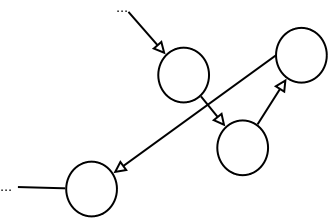
\includegraphics[width=0.3\textwidth]{graphes/2opt1.png}
    \end{center}

    On obtiendrait ceci, en éliminant le croisement:

    \begin{center}
    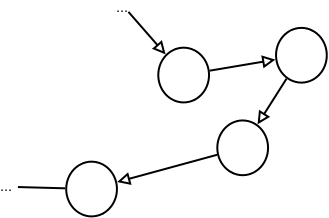
\includegraphics[width=0.3\textwidth]{graphes/2opt2.png}
    \end{center}

    L'algorithme pour le 2-opt est le suivant:
      \begin{lstlisting}
Entrée : un cycle hamiltonien (liste de sommets) et son coût
Sortie : un cycle hamiltonien et son coût inférieur ou égal au coup d'entrée

pour chaque couple de points (a, b) dans le cycle:
    nouveau_coût = coût
                     - "coût de a à son successeur dans le cycle"
                     - "coût de b à son successeur dans le cycle"
                     + "coût de a à b"
                     + "coût du successeur de a et au successeur de b dans le cycle"

    si nouveau_coût < coût:
        coût = nouveau_coût
        cycle = cycle crée en échangeant a et b dans cycle

retourner (coût, cycle)
      \end{lstlisting}

    Il a donc une complexité quadratique du nombre de sommets du cycles.

    L'application du 2-opt sur le chemin obtenu via une heuristique simple peut
    donner des résultats plus proches de la solution optimale qu'on pourrait le
    penser, et la combinaison des deux est donc une bonne méthode.

  \subsubsection{Métaheuristiques}

  Plutôt que d'utiliser une simple heuristique pour trouver une solution à priori plutôt
  bonne, puis d'y appliquer une recherche locale pour tenter de l'améliorer encore,
  il est possible d'utiliser des «~métaheuristiques~».
  Ces algorithmes vont avoir besoin d'heuristiques et de recherche locale, mais vont
  s'en servir en boucle, pour tenter sans cesse de trouver une solution meilleure.

  Ils vont partir explorer différentes parties de l'espace, souvent en guidant
  leur exploration grâce à l'heuristique, et en essayant de retomber sur des
  parties de l'espace les plus intéressantes possibles grâce aux algorithmes de
  recherche locale.

  Il existe énormément de métaheuristiques. En voici quelques uns:
  \begin{description}
  \item[Recherche locale itérée] métaheuristique très simple consistant à
    utiliser une heuristique puis appliquer de la recherche locale pour
    améliorer son résultat.  Ensuite, on perturbe légèrement ce résultat, on
    applique à nouveau une recherche locale et on recommence.
  \item[Recherche tabou] amélioration de la recherche locale itérée, qui va
    utiliser une «~liste taboue~» bannissant toute recherche autour des zones de
    l'espace déjà explorées.
  \item[Recuit simulé] explore d'abord l'espace sans se restreindre aux parties
    donnant des solutions efficaces, puis se restreint de plus en plus au
    voisinage de celles-ci. Converge donc vers les solutions les plus efficaces
    trouvées, puis relâche les contraintes et explore autour de ces dernières,
    quitte à trouver des solutions vraiment moins efficaces. Recommence à se
    contraindre aux plus efficaces, etc\dots
  \item[Algorithmes génétiques] imitent la sélection naturelle, avec une
    population de solutions qui évoluent en mutant et en s'échangeant leurs
    caractéristiques entre elles. On peut même faire évoluer des populations
    séparément avec les modèles en îles, pour avoir plusieurs populations très
    différentes.
  \item[Colonies de fourmis] imitent là encore la nature en simulant des
    phéromones déposées par des fourmis virtuelles, qui orientent la recherche
    au fil du temps.
  \end{description}

  \subsubsection{Conclusion}
    Il est intéressant de constater que les heuristiques, les méthodes de
    recherche locales et les métaheuristiques sont des choses extrêmement
    générales, utilisées pour résoudre énormément de problèmes demandant
    d'explorer un espace extrêmement grand.

    Elles ne sont donc pas propres au voyageur du commerce, même si on a vu
    comment, dans ce cas précis, on pouvait obtenir des résultats corrects en
    se passant de métaheuristiques. On pourrait donc améliorer ces résultats en
    en utilisant.
